% NTCIR-19 FEHU Task 1 working preview.
% Prose source: paper_draft.md
% This file follows the official NTCIR-19 acmart setup and adds the a4paper
% option at the user's request. Placeholder space is deliberate and forms part
% of the eight-page budget check.
\documentclass[sigconf,article,a4paper]{acmart}

\settopmatter{printacmref=false}
\renewcommand\footnotetextcopyrightpermission[1]{}
\pagenumbering{gobble}

\usepackage{amsmath}
\usepackage{array}
\usepackage{booktabs}
\usepackage{float}
\usepackage{placeins}
\usepackage{tabularx}
\usepackage{xcolor}
\usepackage{pgfplots}
\pgfplotsset{compat=1.18}
\geometry{a4paper}
\setlength{\emergencystretch}{1em}
% Keep two-column float glue from stretching into conspicuous blank regions.
\setlength{\textfloatsep}{8pt plus 2pt minus 2pt}
\setlength{\floatsep}{8pt plus 2pt minus 2pt}
\setlength{\intextsep}{8pt plus 2pt minus 2pt}

\definecolor{placeholderbg}{RGB}{247,247,247}
\definecolor{placeholderline}{RGB}{185,185,185}
\newcommand{\placeholdernote}[1]{%
  \par\smallskip
  \noindent\fcolorbox{placeholderline}{placeholderbg}{%
    \parbox{0.94\columnwidth}{\centering\small\color{gray}#1}}
  \par\smallskip
}
\newcommand{\placeholderblock}[2]{%
  \par\smallskip
  \noindent\fcolorbox{placeholderline}{placeholderbg}{%
    \parbox[c][#2][c]{0.94\columnwidth}{%
      \centering\small\color{gray}#1}}
  \par\smallskip
}

\title{WAIPS at the NTCIR-19: Label-Aware Prompt Ensembling and Gated Fusion for Human-Value Recognition}

% TODO(camera-ready): confirm author order, affiliations, countries, and e-mail.
\author{Peiyang Huang}
\affiliation{%
  \institution{Waseda University}
  \country{Japan}
}

\author{Dongyang Liu}
\affiliation{%
  \institution{Waseda University}
  \country{Japan}
}

% TODO(camera-ready): add the remaining confirmed coauthors in the agreed order.

\begin{document}

\begin{abstract}
We present the three official runs submitted to NTCIR-19 FEHU Task 1, which asks
systems to recognize actor-conditioned human values in news and to predict
direction for fine-grained values. Development experiments showed a recurring
trade-off: conservative prompt ensembles preserve direction but miss
infrequent values, whereas recall-oriented methods recover more labels but add
false positives. WAIPS-01 uses label-wise development analysis to determine
which labels a targeted prompt may add to a conservative majority. For
WAIPS-03, we augment difficult directed labels and tune DeBERTa-v3-base with
LoRA and masked partial-label supervision. We combine the resulting encoder
probabilities with heterogeneous prompt jurors through calibrated,
frequency-gated veto and addition rules, followed by focused direction
verification. WAIPS-03
scores 0.5808 Micro-F1 and 0.3952 Macro-F1 on official Task 1b, the highest
Macro-F1 among participant runs. WAIPS-01 has the lowest participant
Direction Reverse Rate (DRR), 0.0345. Targeted augmentation
improves score separation for 18 low-frequency labels, while E6b supplies
direct tail recall. Together, these signals support macro performance under
conservative gates, although the missing final no-DeBERTa ablation prevents
assigning the official gain to one component.
\end{abstract}

\keywords{human values, multi-label classification, long-tail learning, data
augmentation, prompt ensemble, calibrated fusion}

\maketitle
\pagestyle{plain}
\raggedbottom

\section*{Team Name}
WAIPS

\section*{Subtasks}
Task 1a and Task 1b

\section{Introduction}

Human values are often expressed indirectly in news \cite{schwartz2012}. A report may describe the
same decision as protecting public safety for one actor and restricting freedom
for another. Recognizing a value therefore requires more than locating a
topical phrase: the system must identify whose action is being judged, which
value it concerns, and whether the action aligns with or contradicts that
value. FEHU Task 1 defines these decisions explicitly \cite{wangFehu2026}. Task 1a asks for
directionless Level-2 values for each article--actor pair, while Task 1b
evaluates directed Level-1 values. We refer readers to the Task Overview by
Wang et al. for the collection construction, taxonomy, and official evaluation
protocol \cite{wangFehu2026,wangNevu2026}.

Three properties of the task shaped our design. The output space is
strongly imbalanced. A small group of values appears throughout the training
set, while many directed Level-1 classes have only a few examples. This resembles
the long-tail behavior studied in imbalanced classification \cite{cui2019,menon2021}. A system can
therefore obtain reasonable Micro-F1 while never predicting several valid
labels. Increasing recall is also unusually expensive: every extra value
creates another opportunity for both a false positive and a direction
reversal. The available models also make different errors. Prompt variants
make complementary errors, and the encoder can expose weak tail-label evidence
that is not reliable enough to use as a final decision by itself. Our use of
agreement as evidence is related to consistency-based prompting
\cite{wangSelfConsistency2023}, although our rule is an exact-tuple,
label-aware ensemble rather than chain-of-thought self-consistency.

The components are not combined in a single voting rule; each has a distinct
role. WAIPS-01, developed by Liu, starts with a conservative
prompt majority and selectively restores predictions for labels on which a
targeted prompt performed better on development data. A separate augmentation track
diagnoses difficult directed labels, generates focused training cases, and
trains a parameter-efficient DeBERTa classifier to supply continuous evidence.
WAIPS-03 (E7-G4) uses E6b, a recall-oriented prompt system with
self-segmentation, as its primary generator; other prompt runs and the
augmented encoder act as jurors.
A calibrated gate removes weak frequent-class predictions and admits a small
number of supported additions. Direction is then checked only when jurors
explicitly disagree.

We interpret the results according to these roles. E6b supplies much
of the direct tail recall, the DeBERTa track improves representation of
selected low-frequency labels and contributes an auxiliary probability signal,
and the fusion layer controls the precision cost of combining them. We report
both F1 and DRR throughout because the official runs occupy different
points on that trade-off.

\section{Task Setting and Submitted Runs}

For each actor listed in an article, Task 1b requires a set of (Level-1 value,
direction) pairs. We treat the two directions of each of 54 Level-1 values as
108 atomic classes. Task 1a separately evaluates directionless Level-2 values;
the official task definition does not require a system to derive one subtask's
output from the other \cite{wangFehu2026}. Each submitted run therefore uses the
run-specific Task-1a construction described below. Development experiments use
the official 177-article development set. The frozen inference pipelines were
then applied to 175 test articles containing 479 released article--actor pairs;
no test labels or Task-2 annotations were used.

We follow the official evaluator and the Task Overview \cite{wangFehu2026} in treating Micro-F1 as
the primary ranking measure. Macro-F1 is averaged over labels that occur at
least once in the test gold data, making it a useful but support-dependent view
of tail behavior. DRR counts opposite-direction predictions for gold
actor--value pairs with a unique direction. A missed value does not count as a
reversal, so a low DRR must be read together with F1 rather than as a standalone
accuracy measure.

The three submissions use different designs. WAIPS-01 is Liu's
label-aware prompt ensemble, described in Section~\ref{sec:liu}. WAIPS-02 uses
a three-way majority vote over DeepSeek Pro prompt variants and uses a Flash
prediction, when available, to arbitrate direction. WAIPS-03 is the E7-G4
heterogeneous fusion described in Sections~\ref{sec:e7} and~\ref{sec:results}.
This paper focuses on WAIPS-01 and WAIPS-03 because they represent the two main
methodological lines; WAIPS-02 is retained as a prompt-only reference
point.

\begin{table}[H]
  \caption{The three submitted WAIPS runs.}
  \label{tab:runs}
  \small
  \begin{tabularx}{\columnwidth}{@{}lX@{}}
    \toprule
    Run & Short description \\
    \midrule
    WAIPS-01 & Label-aware prompt ensemble; direction-stable selective recovery. \\
    WAIPS-02 & Three-way prompt majority with direction arbitration. \\
    WAIPS-03 & E7-G4 gated heterogeneous fusion. \\
    \bottomrule
  \end{tabularx}
\end{table}

WAIPS-02 is an intermediate prompt-only system. One
DeepSeek Pro prompt is the baseline, one is compact and strict, and one uses
targeted balanced few-shot examples; all run at temperature zero. A label is retained
when at least two runs emit the same actor, value, and direction.
The Flash run is then consulted only for direction: when it predicts the same
actor and value with the opposite direction, the majority direction is
replaced. Task 1a is deterministically projected from the resulting Task-1b
set. Unlike E7-G4, this run has no learned calibrator, encoder features,
frequency gate, or per-cell QA call.

\section{Label-Aware Prompt Ensembling (WAIPS-01)}
\label{sec:liu}

% Replace the five placeholder blocks under
% \section{Label-Aware Prompt Ensembling (WAIPS-01)} with this complete text.
% All figures below are native LaTeX; no external images are required.

\subsection{Method motivation and prompt-only design}

WAIPS-01 is Liu's standalone prompt-only submission and was developed
separately from the later E7-G4 heterogeneous fusion. Development experiments
showed that prompt variants can have complementary error profiles. A strict
evidence requirement makes the system conservative and helps avoid unsupported
values and direction reversals, but it also suppresses
true labels. A targeted prompt recovers difficult values but adds
false positives. We formulate ensembling as a label-specific
selection problem, rather than treating every prompt prediction equally. This
development-set analysis is related to label-wise long-tail diagnosis
\cite{cui2019,menon2021}, but the fixed directed-label set and exact-tuple rule
were determined by our own FEHU development experiments.

We designed the prompt sequence to cover both sides of this trade-off. After
reproducing the A0-style pipeline, we evaluated DeepSeek V4 Flash as a
recall-oriented baseline: its Task-1b recall was .4845, compared
with .2448 for GPT-4o A0. The compact variant removed the reasoning field,
requested only strict JSON, and capped each actor at six values to reduce output
cost and unnecessary explanation. Compact-strict then strengthened the evidence
requirement to create a deliberately conservative member; it reached .6247
precision and .0180 DRR, but only .4255 recall. The later targeted-more-shot
variants addressed the opposite failure mode with additional examples for
difficult health, society, safety, recognition, reputation, and capability
values. The balanced targeted variant was retained as the complementary source
because it recovered more difficult labels without the most aggressive recall
behavior of the earlier targeted prompt.

For an article--actor pair, each prompt returns a structured set of atomic
Task-1b tuples $(a,v,d)$, where $a$ is the actor, $v$ is a Level-1 value, and
$d$ is its aligned or contradictory direction. We use three DeepSeek V4 Flash
variants to form a conservative base: (i) a baseline A0-style prompt, (ii) a
compact prompt that requests concise structured JSON output, and (iii) a
compact-strict prompt with a stronger evidence requirement. A fourth,
targeted-more-shot-balanced prompt is designed as a complementary, higher
recall source using targeted examples for difficult values. All prompt runs
use structured Task-1 outputs and are evaluated with the official evaluator.
This track also includes the end-to-end data, prompting, API, parsing,
prediction, evaluation, and submission-validation pipeline. No model
fine-tuning or learned calibration is used in WAIPS-01.

Figure~\ref{fig:liu-pipeline} summarizes the complete procedure. The
\emph{Liu local} prompt used as one juror in E7-G4 is only one component from
this work; it is not the complete WAIPS-01 method, which includes conservative
voting, label-level diagnosis, and selective addition.

\begin{figure}[t]
  \centering
  \fbox{%
  \begin{minipage}{0.91\columnwidth}
    \centering\small
    \textbf{Article + actor}\\[-1pt]
    $\downarrow$\\[-1pt]
    \textbf{Two parallel Task-1b sources}\\[-1pt]
    Base variants (baseline / compact / compact-strict) $\rightarrow$ exact-tuple majority $M$ ($\geq 2/3$)\\[-1pt]
    Targeted-more-shot-balanced prompt $T$\\[-1pt]
    $\downarrow$\\[-1pt]
    \textbf{Development-only label-level comparison of $M$ and $T$}\\[-1pt]
    \scriptsize (TP, FP, FN, F1, and frequency groups)\\[-1pt]
    $\downarrow$\\[-1pt]
    Fixed set $L$ of ten directed Level-1 labels\\[-1pt]
    $\downarrow$\\[-1pt]
    \textbf{Task 1b selective recovery:} $M$ + $T$ tuples only for labels in $L$\\[-1pt]
    $\downarrow$\\[-1pt]
    Task 1b: recovered directed output \quad | \quad Task 1a: use $T$ output directly
  \end{minipage}}
  \caption{WAIPS-01 uses a conservative exact-tuple majority base and a
  separate targeted prompt. Their development-set comparison fixes the labels
  eligible for Task 1b selective recovery; Task 1a uses the targeted output
  directly.}
  \label{fig:liu-pipeline}
\end{figure}

\subsection{Exact-tuple majority base}

Let $B$, $C$, and $S$ denote the Task-1b prediction sets of the baseline,
compact, and compact-strict variants. We retain an atomic tuple only when at
least two of the three variants agree:
\begin{equation}
 M=\left\{t:\mathbf{1}[t\in B]+\mathbf{1}[t\in C]+\mathbf{1}[t\in S]\geq2\right\}.
 \label{eq:liu-majority}
\end{equation}
The direction is part of $t$. Thus, two prompts that predict the same value
with opposite directions do not support the same tuple. We deliberately use
this precision-oriented exact-tuple rule instead of a value-only vote followed
by separate direction repair. It produces a stable base with development precision 0.6350
and DRR 0.0180, but its recall is only 0.4636 (Table~\ref{tab:liu-dev}).

The error counts show the same trade-off. Relative to the DeepSeek
baseline, majority voting reduced Task-1b false positives from 868 to 637
($-231$), while false negatives increased from 1,232 to 1,282 ($+50$). The
effect was not uniform across the label distribution. Average per-label F1
changed only from .4796 to .4817 for frequent labels and from .2815 to .2866
for medium-frequency labels, but dropped from .2537 to .2168 for infrequent
labels. These results support majority voting as a conservative base, but not
as a complete method: its agreement rule disproportionately removed rare true
positives. This pattern motivated the label-level diagnosis and selective
recovery below.

\subsection{Label-level diagnosis and selection rule}

Aggregate F1 does not show \emph{which} directed values are lost by the
conservative base. We compared majority voting and the targeted
prompt independently for every $(d,v)$ identity on the development set,
recording TP, FP, FN, precision, recall, and F1. We also grouped labels by
their frequency to check whether any aggregate gain was concentrated only on
frequent classes. The diagnosis showed that majority voting made systematic
false-negative errors on a small, interpretable group of values, while the
targeted prompt improved their recall enough to offset its additional false
positives.

We fixed the following ten directed Level-1 identities from this development
comparison. The set is intentionally small: it limits selective addition to
labels with observed complementary behavior rather than opening the final
prediction set to every targeted-prompt output.

\begin{table}[t]
  \caption{Directed labels eligible for selective recovery in WAIPS-01.}
  \label{tab:liu-selected-labels}
  \centering
  \scriptsize
  \begin{tabular}{@{}ll@{}}
    \toprule
    Direction & Level-1 value \\
    \midrule
    Contradictory & Be creative \\
    Contradictory & Have good health \\
    Contradictory & Have a stable society \\
    Contradictory & Have equality \\
    Contradictory & Have harmony with nature \\
    Aligned & Be capable \\
    Aligned & Have good health \\
    Aligned & Have a stable society \\
    Aligned & Be humble \\
    Aligned & Have a world at peace \\
    \bottomrule
  \end{tabular}
\end{table}

Let $T$ be the directed tuple set generated by the
targeted-more-shot-balanced prompt and let $L_{\mathrm{selected}}$ denote the
fixed set in Table~\ref{tab:liu-selected-labels}. The final Task-1b output is
\begin{equation}
 P=M\cup\{t\in T:\operatorname{label}(t)\in L_{\mathrm{selected}}\}.
 \label{eq:liu-selective}
\end{equation}
$M$ remains the default answer; $T$ is allowed to supplement it
only for the chosen directed labels. This method is neither a blind union nor
a weighted or calibrated vote, and it does not use fine-tuning. For Task 1a,
we use the corresponding targeted-more-shot-balanced structured value output,
as submitted in WAIPS-01.

\subsection{Development results and analysis}

Table~\ref{tab:liu-dev} reports the trade-off that motivated the method.
Relative to majority voting, selective recovery increases Task-1b Micro-F1 by
0.0298 and Macro-F1 by 0.0338. The gain is primarily recall: recall rises by
0.0602, compared with a precision decrease of 0.0201. DRR rises from 0.0180 to
0.0279, so recovering more directed values has a measured cost in direction
reversals.

\begin{table}[t]
  \caption{Task-1b development results for Liu's prompt-only variants. A dash
  denotes a metric that was not recorded for that run.}
  \label{tab:liu-dev}
  \centering
  \scriptsize
  \begin{tabular}{@{}lrrrrr@{}}
    \toprule
    Method & Micro & Macro & Prec. & Recall & DRR \\
    \midrule
    GPT-4o A0 & .3424 & .1496 & .5696 & .2448 & .0212 \\
    DeepSeek baseline & .5245 & .3599 & .5716 & .4845 & .0243 \\
    Compact & .5261 & .3511 & .5698 & .4887 & .0261 \\
    Compact-strict & .5062 & .3234 & .6247 & .4255 & \textbf{.0180} \\
    Majority vote & .5359 & .3532 & \textbf{.6350} & .4636 & \textbf{.0180} \\
    Targeted prompt & .5387 & .3679 & .5750 & .5067 & .0302 \\
    Label-aware ensemble & \textbf{.5657} & \textbf{.3870} & .6149 & \textbf{.5238} & .0279 \\
    \bottomrule
  \end{tabular}
\end{table}

For Task 1a on development data, the DeepSeek baseline, compact, and
compact-strict prompts obtained Micro/Macro-F1 of .6490/.5065, .6441/.4871,
and .6125/.4576, respectively. The targeted prompt and the label-aware run both
recorded .6555/.5044 because WAIPS-01 used the targeted structured output for
Task 1a. The majority run recorded .6507 Micro-F1; its remaining Task-1a
metrics were not retained in the experiment log.

The improvement extends beyond frequent labels. The average per-label F1
for the infrequent group rises from 0.2168 to 0.3025, whereas the medium group
is unchanged (Figure~\ref{fig:liu-analysis}(a)). Figure~\ref{fig:liu-analysis}(b)
shows representative cases. For example, contradictory \emph{Have a stable
society} improves from 0.2545 to 0.5611, aligned \emph{Have good health} from
0.3188 to 0.5496, and contradictory \emph{Have harmony with nature} from zero
to 0.8000. These examples are consistent with the intended behavior: selective
recovery addresses known gaps in the conservative ensemble rather than adding
labels uniformly.

\begin{figure}[!t]
  \centering
  {\scriptsize\textbf{(a) Label-frequency analysis}\par}
  {\scriptsize\textcolor{gray!65}{\rule{7pt}{7pt}} DeepSeek baseline\quad
  \textcolor{blue!70!black}{\rule{7pt}{7pt}} Majority vote\quad
  \textcolor{teal!70!black}{\rule{7pt}{7pt}} Label-aware ensemble\par}
  \vspace{.2em}
  \makebox[\columnwidth][c]{%
  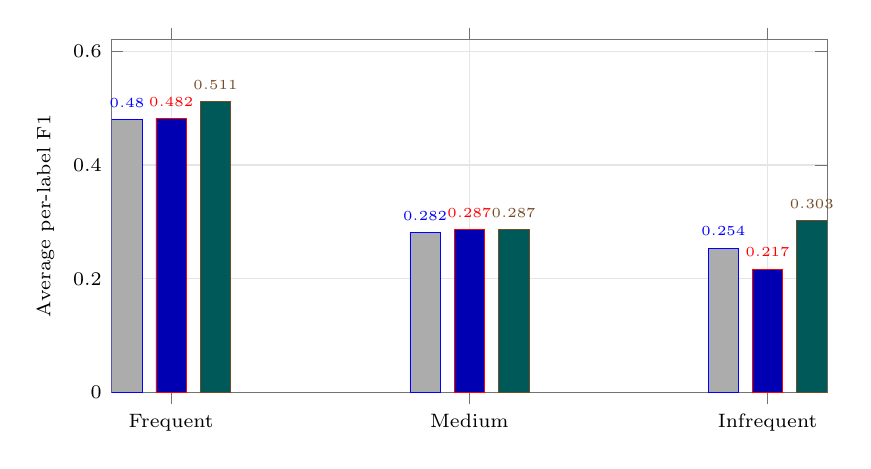
\begin{tikzpicture}
    \begin{axis}[
      width=.88\columnwidth, height=.50\columnwidth,
      ybar=5pt, bar width=11pt,
      ymin=0, ymax=.62,
      ylabel={Average per-label F1},
      symbolic x coords={Frequent,Medium,Infrequent},
      xtick=data,
      x tick label style={font=\scriptsize},
      yticklabel style={font=\scriptsize},
      label style={font=\scriptsize},
      grid=major, grid style={gray!20},
      axis line style={black!55},
      tick style={black!55},
      nodes near coords, nodes near coords style={font=\tiny, /pgf/number format/fixed, /pgf/number format/precision=3, yshift=1pt},
      every axis plot/.append style={draw=black!40, line width=.25pt}
    ]
      \addplot+[fill=gray!65] coordinates {(Frequent,.4796) (Medium,.2815) (Infrequent,.2537)};
      \addplot+[fill=blue!70!black] coordinates {(Frequent,.4817) (Medium,.2866) (Infrequent,.2168)};
      \addplot+[fill=teal!70!black] coordinates {(Frequent,.5109) (Medium,.2866) (Infrequent,.3025)};
    \end{axis}
  \end{tikzpicture}}

  \vspace{.65em}

  {\scriptsize\textbf{(b) Representative label recovery}\par}
  {\scriptsize\textcolor{blue!70!black}{\rule{7pt}{7pt}} Majority vote\quad
  \textcolor{teal!70!black}{\rule{7pt}{7pt}} Label-aware ensemble\par}
  \vspace{.2em}

  \makebox[\columnwidth][c]{%
  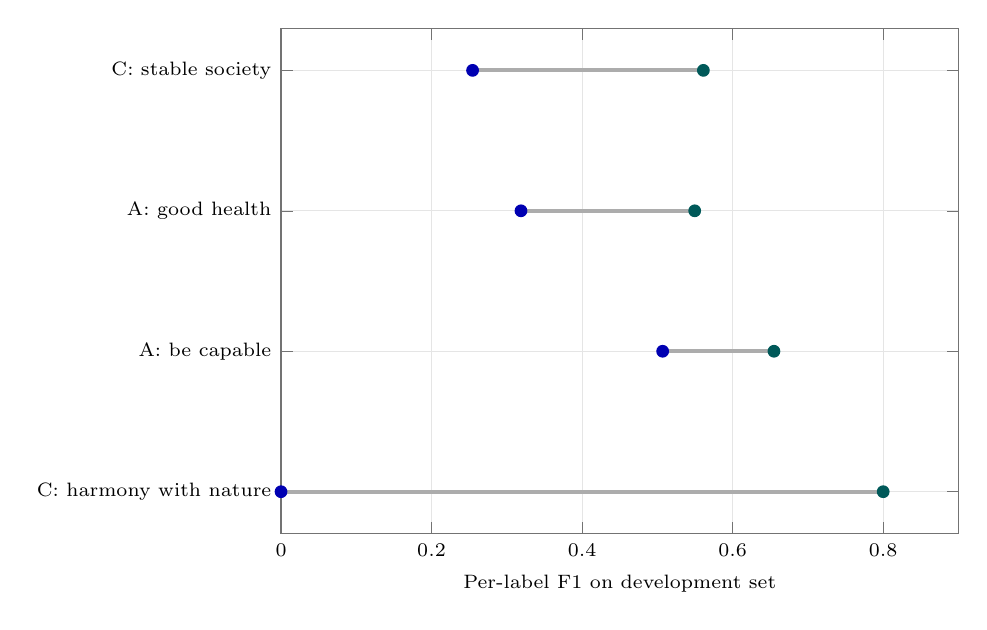
\begin{tikzpicture}
    \begin{axis}[
      width=.84\columnwidth, height=.66\columnwidth,
      xmin=0, xmax=.90,
      xlabel={Per-label F1 on development set},
      ylabel={},
      ytick={1,2,3,4},
      yticklabels={C: stable society,A: good health,A: be capable,C: harmony with nature},
      y dir=reverse,
      yticklabel style={font=\scriptsize, align=right},
      xticklabel style={font=\scriptsize},
      label style={font=\scriptsize},
      grid=major, grid style={gray!20},
      axis line style={black!55},
      tick style={black!55}
    ]
      \addplot[gray!65, line width=1.4pt] coordinates {(.2545,1) (.5611,1)};
      \addplot[gray!65, line width=1.4pt] coordinates {(.3188,2) (.5496,2)};
      \addplot[gray!65, line width=1.4pt] coordinates {(.5070,3) (.6549,3)};
      \addplot[gray!65, line width=1.4pt] coordinates {(.0000,4) (.8000,4)};
      \addplot[only marks, mark=*, mark size=2.1pt, blue!70!black] coordinates {(.2545,1) (.3188,2) (.5070,3) (.0000,4)};
      \addplot[only marks, mark=*, mark size=2.1pt, teal!70!black] coordinates {(.5611,1) (.5496,2) (.6549,3) (.8000,4)};
    \end{axis}
  \end{tikzpicture}}
  \caption{Development-set evidence for diagnosis-guided selective recovery.
  (a) Majority voting slightly improves frequent and medium labels over the
  DeepSeek baseline but harms infrequent labels; selective recovery reverses
  that loss. (b) The method
  recovers selected directed labels without adding every targeted-prompt tuple;
  C and A denote contradictory and aligned, respectively.}
  \label{fig:liu-analysis}
\end{figure}

We also tested smaller subsets of the same ten labels using cached predictions,
without additional LLM calls. Removing the low-impact label \emph{aligned: Be
humble} (ID 1:35; \texttt{small\_best9})
gave .5656 Micro-F1, .3851 Macro-F1, .6150 precision, .5234 recall, and .0279
DRR. Removing \emph{aligned: Have a stable society} (ID 1:27), the label most
associated with direction errors (\texttt{small\_low\_drr}), gave .5613
Micro-F1, .3858 Macro-F1, .6222
precision, .5113 recall, and \textbf{.0230 DRR}. The .0230 result therefore
comes from a final pre-submission development experiment, but it was a
lower-DRR backup rather than the selected submission: the original ten-label
setting retained the best Micro-F1 (.5657) with .0279 DRR.

\subsection{Official result and limitation}

WAIPS-01 was submitted as the direction-stable WAIPS run. On the official test,
it achieved .6589 Micro-F1 and .5366 Macro-F1 on Task 1a, and .5543 Micro-F1,
.3277 Macro-F1, and .0345 DRR on Task 1b. The last value is the lowest DRR
among participant runs \cite{wangFehu2026}. These results support using this run
as a conservative alternative but do not establish dominance on every metric.
The selection set was chosen on development data, and the development and
official test sets contain different articles; consequently, the development
comparison should not be read as a controlled test-time ablation.

The official precision/recall pairs were .6731/.6453 for Task 1a and
.5991/.5157 for Task 1b. The submitted files contained 1,811 Task-1a labels and
2,058 directed Task-1b labels; 264 Task-1b predictions were selectively supplied
by the targeted source. Before packaging, we verified complete article coverage,
released actor membership, taxonomy validity, and the absence of duplicate
tuples for the full development candidate; the corrected test submission used
the same frozen construction and the required two-file Task-1 package structure.
These checks reduce the likelihood that malformed output, rather than the
intended label-aware pipeline, explains the reported result.

We treat the cross-split pattern as descriptive rather than as a controlled
ablation. Task-1b Micro-F1 changed modestly from .5657 on development data to
.5543 on the official test, whereas Macro-F1 fell from .3870 to .3277 and DRR
rose from .0279 to .0345. This suggests weaker generalization for rare or difficult
directed labels than for the aggregate prediction set. The lowest participant
DRR indicates comparatively stable direction assignment, but it does not imply
that rare-label recovery is solved. Because development and test
contain different articles and gold distributions, these differences are
descriptive evidence rather than estimates of a causal generalization gap
\cite{wangFehu2026}.

\section{Diagnosis-Guided Augmentation for Rare-Label Evidence}
\label{sec:augmentation}

\subsection{From label diagnosis to generation targets}

Our initial DeBERTa classifier used a 108-dimensional sigmoid head and a single
global threshold. Per-label analysis showed that this model had effectively
learned no usable ordering for many low-frequency directed labels. We selected
targets at the directed Level-1 class evaluated by Task 1b, rather
than augmenting undirected values uniformly. A class was eligible when its
official training count was at most 130 and its
development support was at least three. Ranking the eligible classes by
diagnostic evidence produced 18 frozen targets: 14 contradictory and four
aligned classes, spanning 12 Level-2 groups.

The data were constructed in two rounds. Synthetic augmentation is widely used
to improve sparse NLP supervision \cite{feng2021}; here we use it only for
diagnosed directed FEHU labels rather than applying generic text perturbations.
Round 1 covered six Level-1 values in
both directions. DeepSeek V4 Pro generated 422 candidates; deterministic checks
and an independent LLM semantic screen retained 340 silver records. These
records were machine-screened, not manually verified. Round 2 concentrated on
the 18 directed targets and allocated exactly 50 records to each target. Its
900 records mix targeted in-context generation, direction contrast cases,
situation transformations, and hard negatives (Table~\ref{tab:generation}).
The hard-negative group includes 36
explicitly known negative labels. All Round-2 records passed schema, taxonomy,
actor mention, direction, and duplicate checks, but they did not receive
semantic LLM screening or human review. We report this provenance distinction
because it limits what can be claimed about data quality.

\begin{table}[H]
  \caption{Round-2 generation strategies.}
  \label{tab:generation}
  \scriptsize
  \begin{tabularx}{\columnwidth}{@{}XrX@{}}
    \toprule
    Strategy & $n$ & Supervision and purpose \\
    \midrule
    Targeted ICL & 450 & Full multi-label; varied contexts and co-values. \\
    Direction contrast & 180 & Target-only; 90 aligned/contradictory pairs. \\
    Transformation & 180 & Target-only; different actor, action, or setting. \\
    Hard negative & 90 & Target-only; 36 explicit negative labels. \\
    \bottomrule
  \end{tabularx}
\end{table}

Generation used explicit constraints rather than free-form paraphrasing.
Each request fixed the actor, target identity, direction, and a news-style
evidence requirement. Local validators rejected malformed mappings, absent
actors, unsupported evidence sentences, forbidden meta-language, and
duplicates before a record could enter the training data. The generation gates
rejected and regenerated 67 Round-1 and 472 Round-2 candidates; the later
Round-1 semantic screen separately excluded 82 of 422 records. Structural gates
establish format and internal consistency; they do not show that every
synthetic label is correct.

\subsection{Partial-label training}

The final training set contains 1,228 official articles, 340 Round-1 records,
and 900 Round-2 records: 2,468 articles and 4,575 actor examples in total.
The synthetic news vignettes are often only partially annotated. Treating every
unlisted class as negative would create hundreds of false-negative training
signals, especially for the single-target records. We mark 3,785 examples as
fully supervised and 790 as target-only. For a target-only
example, binary cross entropy is evaluated only on its known positive entries
and any explicitly known negatives; the remaining label positions receive a
zero loss mask.

We fine-tune DeBERTa-v3-base \cite{he2021} with LoRA adapters \cite{hu2022} on the query
and value projections ($r=16$, $\alpha=32$, dropout 0.1) and a 108-way
classification head. Each input pairs the article text with the actor name and
uses a maximum length of 512. We optimize the model with class-weighted binary
cross entropy. The positive weight for each class is
$\sqrt{n_{\mathrm{negative}}/n_{\mathrm{positive}}}$, clipped to $[1,10]$ and
computed over supervised entries only. We select checkpoints by development
Task-1b Micro-F1 and decode predictions at a global threshold of 0.30. In
E7-G4, the encoder never assigns the final direction: we export all 108 sigmoid
probabilities and use them only as continuous jury features.

For example $i$ and directed class $k$, let $m_{ik}$ be one for an observed
label decision and zero for an unknown entry. Training minimizes
\begin{equation}
\mathcal{L}=\frac{\sum_{i,k}m_{ik}w_k\operatorname{BCE}(y_{ik},z_{ik})}
{\sum_{i,k}m_{ik}}.
\end{equation}
All mask entries are one for official and fully labelled records. On
target-only records, only the intended positives and explicitly supplied hard
negatives contribute. This does not rebalance the dataset to 50:50; it prevents
missing synthetic annotations from becoming certain negatives. The distinction
matters in a 108-class problem, where a single partially annotated example
would otherwise create more than one hundred negative loss terms.

\subsection{What the augmentation did---and did not---establish}

On the 18 targets, mean target AUC with official data only was 0.536, and mean
per-target oracle F1 was 0.053. The augmented v2 checkpoint raised these values
to 0.697 and
0.112; AUC improved for 14 of 18 targets and oracle F1 for 16 of 18. Thus the
generated supervision changed the ranking of target positives, rather than
merely shifting an unchanged distribution across the 0.30 threshold.

\begin{table}[t]
  \caption{Score-level tail diagnostics on development data.}
  \label{tab:tail}
  \small
  \begin{tabular}{@{}lrr@{}}
    \toprule
    Diagnostic & Official & Augmented v2 \\
    \midrule
    Mean AUC (18 targets) & .536 & \textbf{.697} \\
    Mean oracle F1 & .053 & \textbf{.112} \\
    AUC $\leq .55$ & 11/18 & \textbf{3/18} \\
    \bottomrule
  \end{tabular}
\end{table}

The three-seed comparison, which isolates the 900 Round-2 records, shows the
same pattern: the official-only condition remains close to chance
(mean target AUC 0.513), whereas the 900 records raise AUC to 0.624 with
assume negative supervision and 0.577 with masking. Both improvements have the
same sign for all three matched seeds. With the complete 340+900 data, masked
supervision was retained because it had the better mean full-data result and
protected the sparsely annotated Round-1 records; its mean target AUC was
0.632, but with a standard deviation of 0.105.

\begin{table}[t]
  \caption{Three-seed target analysis (mean $\pm$ SD).}
  \label{tab:seeds}
  \small
  \begin{tabular}{@{}lrr@{}}
    \toprule
    Training condition & AUC & Oracle F1 \\
    \midrule
    Official only & $.513\pm.030$ & $.048\pm.010$ \\
    +900, assume negative & $\mathbf{.624\pm.011}$ & $\mathbf{.095\pm.014}$ \\
    +900, masked & $.577\pm.028$ & $.080\pm.019$ \\
    +340+900, masked & $.632\pm.105$ & $.111\pm.049$ \\
    \bottomrule
  \end{tabular}
\end{table}

The gain does not establish a reliable tail classifier. Three
full-data seeds showed substantial variance: target true positives were 0, 0,
and 37, and overall Macro-F1 ranged from 0.022 to 0.182. Given this variance,
the encoder is an auxiliary source rather than a submitted standalone model.
We also describe the final macro result as a joint effect of tail-oriented
generation, E6b's direct recall, and gated fusion. A clean final-fusion
ablation without DeBERTa is not available, so the official E7-G4 gain cannot be
assigned causally to augmentation alone.

\section{E7-G4: Frequency-Gated Heterogeneous Fusion}
\label{sec:e7}

\subsection{Members with deliberately different roles}

E7-G4 starts from E6b, a prompt pipeline that first segments an article into
six to nine coherent developments and then predicts values for each actor using
a fixed few-shot scaffold. Although limited to segmentation granularity, this
change affected development performance. Its predecessor E6 produced a median
of 12 segments and achieved
high recall with many false positives. Asking the segmenter to merge closely
related sentences reduced the median to eight. On development data, E6b
improved over E6 from 0.5412 to 0.5496 Micro-F1 and from 0.4079 to 0.4124
Macro-F1. Relative to the earlier E1 prompt run, its Micro-F1 changed only
slightly (0.5480 to 0.5496), but Macro-F1 rose by 0.0405. We therefore use E6b
as the primary generator because it provides broad coverage that a later fusion
stage cannot supply on its own.

The jurors serve different roles. E1 uses a balanced article-level prompt,
whereas E6 uses finer self-segmentation to favor recall. E6c runs DeepSeek Pro
without thinking over the E6b segments. It has the strongest individual
Task-1a development result (0.6774) but weak direction behavior; we use it as
value evidence, not as a direction authority. The local Liu component is one
targeted balanced few-shot prompt run and is distinct from the
complete label-aware WAIPS-01 method in Section~\ref{sec:liu}. The
augmented DeBERTa model contributes continuous probabilities rather than
discrete predictions.

\begin{table}[t]
  \caption{Development profiles and assigned E7 roles. ``Liu local prompt''
  denotes one targeted juror, not the complete WAIPS-01 ensemble.}
  \label{tab:members}
  \scriptsize
  \begin{tabularx}{\columnwidth}{@{}lrrX@{}}
    \toprule
    Member & Micro/Macro & DRR & E7 role \\
    \midrule
    E1 & .5480/.3719 & .0347 & Balanced juror \\
    E6 & .5412/.4079 & .0504 & Recall juror \\
    \textbf{E6b} & \textbf{.5496/.4124} & .0459 & Primary generator \\
    E6c & .5343/.3725 & .0657 & Value/disagreement juror \\
    Liu local prompt & .5347/.3385 & \textbf{.0230} & Precision juror \\
    DeBERTa & --- & --- & Continuous evidence \\
    \bottomrule
  \end{tabularx}
\end{table}

\begin{figure}[t]
  \centering
  \fcolorbox{placeholderline}{white}{%
    \begin{minipage}{0.91\columnwidth}
      \centering\small
      Article + actor\\[2pt]
      $\downarrow$\\[-1pt]
      E6b primary predictions\\[2pt]
      $\searrow$\hspace{22pt}$\swarrow$\\[-1pt]
      \begin{tabular}{c@{\hspace{10pt}}c}
        E1 / E6 / E6c / Liu & DeBERTa probabilities
      \end{tabular}\\[2pt]
      $\downarrow$\\[-1pt]
      Calibrated veto + capped additions (G3)\\[2pt]
      $\downarrow$\\[-1pt]
      Disagreement-triggered direction QA (G4)\\[2pt]
      $\downarrow$\\[-1pt]
      Task-1b $\rightarrow$ deterministic Task-1a projection
    \end{minipage}}
  \caption{E7-G4 separates value generation, calibrated fusion, and direction repair.}
  \Description{The E6b primary predictions, four prompt jurors, and DeBERTa
  probabilities feed calibrated veto and addition rules, followed by focused
  direction quality assurance and deterministic Task-1a projection.}
  \label{fig:e7}
\end{figure}

\subsection{Calibrated veto and additions}

For an actor and directed value cell $c$, the removal score combines
exact-direction votes, value-only votes, and the encoder's directionless value
score:
\begin{equation}
s_{\mathrm{rm}}(c)=n_{\mathrm{exact}}(c)+0.25n_{\mathrm{value}}(c)
 +p_D(\mathrm{value}(c)).
\end{equation}
For a candidate not emitted by E6b, the addition score is stricter:
\begin{equation}
s_{\mathrm{add}}(c)=n_{\mathrm{exact}}(c)+p_D(c).
\end{equation}
Pool-adjacent-violators calibration maps each monotone score to an empirical
probability of being gold. During development, calibration is two-fold
cross-fitted by article, so an article's own labels do not determine its
mapping. This monotone score-calibration approach follows the established use
of isotonic regression for classifier probabilities \cite{zadrozny2002}. For
test inference, the mapping is fitted once on the full development
set and applied unchanged. The decision threshold follows the plug-in
expected-F1 rule, $\tau=F1_{\mathrm{primary}}/2$; the frozen full-development
value is 0.27479.

The rules are intentionally asymmetric. A primary cell is removed only when
its calibrated probability is below $\tau$, it belongs to one of 38 frequent
directed classes (official training count greater than 130), and the actor
retains at least one label. A non-primary cell can be added only when it was
proposed by a juror, its calibrated probability reaches $\tau$, it is in the
same frequent tier, and E6b does not already hold the value in either direction.
Additions are capped at two per actor. In the ungated development control,
removing weak tail predictions reduced Macro-F1 sharply. The frequency gate
also means that the 18 augmentation targets are not directly
switched on or off by the G3 actions; the encoder supplies broader score
evidence, while E6b remains the main direct source of tail labels.

\subsection{Focused direction repair}

The last stage addresses direction errors separately. A fused prediction is sent to
direction QA only if at least one juror predicts the same value in the opposite
direction and the fused set does not already contain both directions. DeepSeek
Flash then receives the article, actor, and one value and returns only
\texttt{aligned} or \texttt{contradictory}. On development data, 176 cells were
flagged and 46 were flipped; seven failed all retries and were retained with
explicit failure records. On test, 207 cells were flagged, 77 were flipped,
and five failed and were retained. Because this stage never introduces a new
value, it can repair direction without reopening the value-selection problem.

\subsection{Frozen development-to-test transfer}

The complete test path was executed as a fit--apply procedure. All prompt
members read only the official Task-1 test article file; E6 and E6b generated
their own segmentations because official test subevents were unavailable. The
removal and addition calibrators were fitted on all development data and loaded
unchanged for test. We also froze the frequency tier, score weights, threshold,
maximum of two additions, and QA trigger. Every empty API response or parsing
failure was retried. If retries were exhausted, the failure either stopped the
stage or, under the predeclared QA behavior, was logged while retaining the
original direction.

Before submission, both files were checked for complete article coverage,
valid actor membership, taxonomy ranges, duplicate tuples, and deterministic
Task-1a projection. The final WAIPS-03 output contained 2,764 directed labels,
covering 93 of the 108 classes and all 54 Level-1 values. These counts cannot
substitute for test labels, but the removal/addition profile was close to
development and gave no operational indication of a broken transfer pipeline.

\section{Experiments and Results}
\label{sec:results}

\subsection{Development results}

Table~\ref{tab:dev} reports the successive stages of E7-G4. E6b already raises
Macro-F1 by 0.0405 over E1. This initial gain matters when interpreting the
final macro-F1 result. The calibrated veto (G1) mainly restores precision.
Re-enabling supported additions (G3) provides the largest single fusion
increment, and direction QA (G4) produces a smaller but consistent improvement
in Micro-F1, Macro-F1, and DRR.

\begin{table}[H]
  \caption{Development results. T18 is Micro-F1 over the 18 augmentation targets.}
  \label{tab:dev}
  \centering
  \resizebox{\columnwidth}{!}{%
  \begin{tabular}{@{}lrrrrrr@{}}
    \toprule
    System & 1b Micro & Precision / Recall & 1b Macro & 1a Micro & DRR & T18 \\
    \midrule
    E1 & .5480 & .541 / .556 & .3719 & .6574 & .0347 & .2460 \\
    E6b primary & .5496 & .502 / .608 & .4124 & .6621 & .0459 & .3145 \\
    G1: calibrated veto & .5608 & .559 / .563 & .4146 & .6587 & \textbf{.0374} & .3145 \\
    G3: veto + additions & .5790 & .539 / .626 & .4266 & .6874 & .0450 & .3145 \\
    \textbf{G4: G3 + direction QA} & \textbf{.5817} & \textbf{.542 / .629} & \textbf{.4308} & \textbf{.6874} & .0419 & \textbf{.3264} \\
    \bottomrule
  \end{tabular}}
\end{table}

The G4--E6b Micro-F1 difference is 0.0321. In a paired article bootstrap with
10,000 resamples, the 95\% interval runs from 0.0209 to 0.0433. This interval
measures article-sampling variation; it does not measure nondeterminism across
LLM calls. G1 removed 484 predictions on development data and
G3 admitted 364. The test pipeline was frozen before inference and produced a
similar action profile: 529 removals and 365 additions. These counts are useful
for checking operational consistency, not for estimating test-set quality.

Two controls help explain the final gated rule. Removing the local Liu prompt
from the veto jury changes Micro-F1 from .5608 to .5619. This control concerns
only that single E7-G4 juror; it is not an ablation of Liu's complete WAIPS-01
label-aware ensemble in Section~\ref{sec:liu}. The juror's precision-oriented
profile is more relevant when additions are considered. Conversely, allowing
vetoes on all classes gives 0.5703 Micro-F1
but only 0.3900 Macro-F1. This is the failure mode the frequency gate was
designed to prevent: a weak auxiliary score can appear favorable in aggregate
by suppressing difficult labels that macro-F1 is intended to expose.

\subsection{Where the macro gain enters}

The development results localize the Macro-F1 gains more precisely than the
final-run comparison alone. Moving from E1 to E6b raises Macro-F1 from 0.3719
to 0.4124 (+0.0405) while changing Micro-F1 by only +0.0016. The
frequent-class veto then adds +0.0022 Macro-F1, supported additions add a
further +0.0120, and
direction QA adds +0.0042. The 18-target Micro-F1 is 0.3145 for E6b and remains
unchanged through G1 and G3; direction QA raises it to 0.3264.

This decomposition is consistent with the assigned roles. E6b directly emits
most of the additional tail labels. Augmentation improves
rare-label separation in the DeBERTa score space and contributes a continuous
confidence signal, but the frequent-class gate prevents G3 from directly
adding the 18 selected targets. Its support for the final macro-oriented system
is therefore indirect and shared with the prompt jury. We regard the official
macro advantage as consistent with the combined design, not as a demonstration
that augmented DeBERTa alone caused it.

\subsection{Official results}

The Task Overview \cite{wangFehu2026} reports four evaluated run packages from two teams: three
from WAIPS and one from IIUoT. The results show different trade-offs rather than
one uniformly dominant run. WAIPS-02 gives our highest Task-1a Micro-F1,
WAIPS-03 gives our strongest Task-1b Micro- and Macro-F1, and WAIPS-01 gives the
lowest DRR among participant runs. Across teams, IIUoT-01 leads the primary
Micro-F1 ranking on Tasks 1a and 1b, while WAIPS-03 has the highest participant
Task-1b Macro-F1. The organizer baseline is an unranked reference and exceeds
every participant run on Task-1b Micro- and Macro-F1. We state the
macro result as a participant comparison, not as overall task dominance.

\begin{table}[!t]
  \caption{Official Task-1 results. Each F1 entry is Micro / Macro. The
  organizer baseline is unranked; bold marks the best participant.}
  \label{tab:official}
  \centering
  \scriptsize
  \resizebox{\columnwidth}{!}{%
  \begin{tabular}{@{}lrrr@{}}
    \toprule
    System / run & Task 1a F1 & Task 1b F1 & DRR \\
    \midrule
    Organizer baseline & .6782 / .5405 & .6284 / .4402 & .0386 \\
    IIUoT-01 & \textbf{.7042 / .5808} & \textbf{.5979} / .3930 & .0613 \\
    WAIPS-01 & .6589 / .5366 & .5543 / .3277 & \textbf{.0345} \\
    WAIPS-02 & .6930 / .5646 & .5496 / .3580 & .0395 \\
    \textbf{WAIPS-03} & .6862 / .5705 & .5808 / \textbf{.3952} & .0477 \\
    \bottomrule
  \end{tabular}}
\end{table}

The development and official results show the same broad, though not fully
uniform, pattern. Broad value recovery helps macro-F1, but it increases
exposure to direction mistakes. WAIPS-01 is the conservative end of this
spectrum. E7-G4 accepts a higher DRR in exchange for more labels and higher
Task-1b F1. Its
targeted direction QA reduces the development reversal rate after additions,
but does not erase the underlying coverage--direction trade-off on the official
test set.

\subsection{Error patterns and limitations}

We observed two recurring error types. The first is over-generation of
plausible values for a nearby actor or for the article in general.
Self-segmentation makes more local evidence visible, but a value can still be
attached to an actor who is mentioned
rather than responsible. The calibrated veto repairs some of these errors only
in frequent classes. The second is direction ambiguity. Jurors often agree that
a value is relevant while disagreeing about whether the actor supports or
undermines it; focused QA helps, but ambiguous reporting and multiple actions
by one actor remain difficult.

Several limitations affect this interpretation. The fusion
weights, frequency gate, and threshold family were designed through analysis of
development data, even though calibration was cross-fitted and the test
pipeline was frozen. The Round-2 synthetic data were structurally checked but
not semantically screened, and masked DeBERTa training has high seed variance.
The final fusion was not rerun in a controlled no-DeBERTa
condition, so the augmentation track's causal share of the official macro
result is unknown. The available evidence shows that it improves low-frequency
score separation and provides auxiliary evidence; E6b and the LLM jury remain
essential. Results from two participating teams should not be read as
a broad leaderboard conclusion.

\FloatBarrier
\section{Related Work}

\textbf{Computational human-value recognition.}
The FEHU taxonomy ultimately builds on the refined theory of basic individual
values \cite{schwartz2012}. Earlier computational resources operationalized
values in arguments \cite{kiesel2022,valueEval2023}, dialogue
\cite{qiu2022}, pluralistic scenarios \cite{sorensen2024}, and broad model
evaluation \cite{ren2024}. These resources provide label spaces, but
factual news requires attribution to a particular actor and grounding across a
long document. NEVU introduced actor-conditioned, direction-aware value
recognition at multiple event granularities \cite{wangNevu2026}; FEHU converts
that setting into four shared-task subtasks and an official evaluation protocol
\cite{wangFehu2026}.

\textbf{Event and actor grounding in news.}
Our use of complete articles and actor-specific outputs is related to work on
event-based news narratives \cite{norambuena2023}, document-level event
arguments \cite{li2021}, and event-extraction benchmarking
\cite{huang2024}. Quotation attribution \cite{zhang2022} and framing analysis
\cite{tohidi2025} likewise show why evidence and agency should not be collapsed
into one article-level judgment. FEHU fixes the actors and evaluation units, so
our contribution is not a new event extractor; it is a set of prediction and
fusion strategies for the released actor-conditioned task.

\textbf{Ensembling, imbalance, and calibrated auxiliary models.}
Consistency-based prompting can improve reliability by aggregating multiple
reasoning paths \cite{wangSelfConsistency2023}. WAIPS-01 differs by voting on
exact structured tuples and permitting selective recovery only for directed
labels diagnosed on development data. This label-aware restriction is motivated
by the long-tail behavior studied in class-balanced and logit-adjusted learning
\cite{cui2019,menon2021}. The second WAIPS line uses targeted synthetic data, a
common response to sparse NLP supervision \cite{feng2021}, and a
DeBERTa/LoRA auxiliary encoder \cite{he2021,hu2022}. E7-G4 then calibrates
monotone ensemble scores with isotonic regression \cite{zadrozny2002}. This
prior work provides context for the components; the FEHU-specific prompt designs,
directed-label diagnostics, and gate configurations were developed in this
project.

\section{Conclusion}

Our Task-1 systems were built by treating label recovery, precision control,
and direction assignment as separate problems. Liu's WAIPS-01 method uses
label-level diagnosis to recover selected misses without abandoning a
conservative prompt majority. The augmentation track gives a LoRA-tuned
DeBERTa encoder substantially better score-level separation on selected rare
directed labels, while E6b supplies strong direct tail recall through
granularity-controlled self-segmentation. E7-G4 combines these heterogeneous
signals with calibrated, frequency-gated veto and addition rules and repairs
direction only where jurors disagree. The official results reflect the
intended trade-off: WAIPS-03 reaches 0.5808 Micro-F1 and 0.3952 Macro-F1 on
Task 1b, while WAIPS-01 remains more direction-stable. The next steps are a
clean component ablation and more stable tail training.

\begin{thebibliography}{99}

\bibitem{wangFehu2026}
Yao Wang, Zhuochen Liu, Jiankang Chen, Haitao Yu, Xin Liu, Kyoungsook Kim,
and Adam Jatowt. 2026.
Overview of the NTCIR-19 FEHU Task: Fact-based Event-centric Human-value
Understanding. In \emph{Proceedings of the 19th NTCIR Conference}.

\bibitem{wangNevu2026}
Yao Wang, Xin Liu, Zhuochen Liu, Jiankang Chen, Adam Jatowt, Kyoungsook Kim,
Noriko Kando, and Haitao Yu. 2026.
Event-Centric Human Value Understanding in News-Domain Texts: An
Actor-Conditioned, Multi-Granularity Benchmark.
\emph{arXiv preprint arXiv:2603.17838}.

\bibitem{schwartz2012}
Shalom H. Schwartz, Jan Cieciuch, Michele Vecchione, Eldad Davidov, Ronald
Fischer, Constanze Beierlein, Alice Ramos, Markku Verkasalo, Jan-Erik
L\"onnqvist, Kursad Demirutku, et al. 2012.
Refining the Theory of Basic Individual Values.
\emph{Journal of Personality and Social Psychology} 103, 4 (2012), 663--688.

\bibitem{kiesel2022}
Johannes Kiesel, Milad Alshomary, Nicolas Handke, Xiaoni Cai, Henning
Wachsmuth, and Benno Stein. 2022.
Identifying the Human Values behind Arguments.
In \emph{Proceedings of ACL 2022}, 4459--4471.

\bibitem{qiu2022}
Liang Qiu, Yizhou Zhao, Jinchao Li, Pan Lu, Baolin Peng, Jianfeng Gao, and
Song-Chun Zhu. 2022.
ValueNet: A New Dataset for Human Value Driven Dialogue System.
In \emph{Proceedings of AAAI 2022}, 11183--11191.

\bibitem{valueEval2023}
Johannes Kiesel, Milad Alshomary, Nailia Mirzakhmedova, Maximilian Heinrich,
Nicolas Handke, Henning Wachsmuth, and Benno Stein. 2023.
SemEval-2023 Task 4: ValueEval: Identification of Human Values behind Arguments.
In \emph{Proceedings of SemEval-2023}, 2287--2303.

\bibitem{sorensen2024}
Taylor Sorensen, Liwei Jiang, Jena D. Hwang, Sydney Levine, Valentina Pyatkin,
Peter West, Nouha Dziri, Ximing Lu, Kavel Rao, Chandra Bhagavatula, et al. 2024.
Value Kaleidoscope: Engaging AI with Pluralistic Human Values, Rights, and
Duties. In \emph{Proceedings of AAAI 2024}, 19937--19947.

\bibitem{ren2024}
Yuanyi Ren, Haoran Ye, Hanjun Fang, Xin Zhang, and Guojie Song. 2024.
ValueBench: Towards Comprehensively Evaluating Value Orientations and
Understanding of Large Language Models.
In \emph{Proceedings of ACL 2024}, 2015--2040.

\bibitem{norambuena2023}
Brian Felipe Keith Norambuena, Tanushree Mitra, and Chris North. 2023.
A Survey on Event-based News Narrative Extraction.
\emph{ACM Computing Surveys} 55, 14s (2023), Article 300, 1--39.

\bibitem{li2021}
Sha Li, Heng Ji, and Jiawei Han. 2021.
Document-Level Event Argument Extraction by Conditional Generation.
In \emph{Proceedings of NAACL-HLT 2021}, 894--908.

\bibitem{huang2024}
Kuan-Hao Huang, I-Hung Hsu, Tanmay Parekh, Zhiyu Xie, Zixuan Zhang, Prem
Natarajan, Kai-Wei Chang, Nanyun Peng, and Heng Ji. 2024.
TextEE: Benchmark, Reevaluation, Reflections, and Future Challenges in Event
Extraction. In \emph{Findings of ACL 2024}, 12804--12825.

\bibitem{zhang2022}
Yuanchi Zhang and Yang Liu. 2022.
DirectQuote: A Dataset for Direct Quotation Extraction and Attribution in News
Articles. In \emph{Proceedings of LREC 2022}, 6959--6966.

\bibitem{tohidi2025}
Amir Tohidi, Samar Haider, and Duncan J. Watts. 2025.
Rethinking News Framing with Large Language Models.
\emph{Scientific Reports} (2025).

\bibitem{wangSelfConsistency2023}
Xuezhi Wang, Jason Wei, Dale Schuurmans, Quoc V. Le, Ed H. Chi, Sharan
Narang, Aakanksha Chowdhery, and Denny Zhou. 2023.
Self-Consistency Improves Chain of Thought Reasoning in Language Models.
In \emph{Proceedings of ICLR 2023}.

\bibitem{cui2019}
Yin Cui, Menglin Jia, Tsung-Yi Lin, Yang Song, and Serge Belongie. 2019.
Class-Balanced Loss Based on Effective Number of Samples.
In \emph{Proceedings of CVPR 2019}, 9268--9277.

\bibitem{menon2021}
Aditya Krishna Menon, Sadeep Jayasumana, Ankit Singh Rawat, Himanshu Jain,
Andreas Veit, and Sanjiv Kumar. 2021.
Long-tail Learning via Logit Adjustment.
In \emph{Proceedings of ICLR 2021}.

\bibitem{feng2021}
Steven Y. Feng, Varun Gangal, Jason Wei, Sarath Chandar, Soroush Vosoughi,
Teruko Mitamura, and Eduard Hovy. 2021.
A Survey of Data Augmentation Approaches for NLP.
In \emph{Findings of ACL-IJCNLP 2021}, 968--988.

\bibitem{he2021}
Pengcheng He, Xiaodong Liu, Jianfeng Gao, and Weizhu Chen. 2021.
DeBERTa: Decoding-enhanced BERT with Disentangled Attention.
In \emph{Proceedings of ICLR 2021}.

\bibitem{hu2022}
Edward J. Hu, Yelong Shen, Phillip Wallis, Zeyuan Allen-Zhu, Yuanzhi Li,
Shean Wang, Lu Wang, and Weizhu Chen. 2022.
LoRA: Low-Rank Adaptation of Large Language Models.
In \emph{Proceedings of ICLR 2022}.

\bibitem{zadrozny2002}
Bianca Zadrozny and Charles Elkan. 2002.
Transforming Classifier Scores into Accurate Multiclass Probability Estimates.
In \emph{Proceedings of KDD 2002}, 694--699.

\end{thebibliography}

\end{document}
